
\documentclass[bwprint]{gmcmthesis}
\usepackage{amsmath}
\usepackage{booktabs}
\usepackage{longtable}
\usepackage{tabularx}
\usepackage{array}
\usepackage{float}
\numberwithin{figure}{section}
\numberwithin{table}{section}
\renewcommand{\thefigure}{\arabic{section}-\arabic{figure}}
\renewcommand{\thetable}{\arabic{section}-\arabic{table}}
\graphicspath{{../figures/}{figures/}}

\title{统一口径下绿电直连型电氢氨园区优化运行研究}
\baominghao{No.00000000}
\schoolname{待填写}
\membera{待填写}
\memberb{待填写}
\memberc{待填写}

\begin{document}
\maketitle

\begin{abstract}
本文面向绿电直连型电氢氨园区优化运行问题，围绕风光出力、常规负荷、电解制氢、合成氨生产、电网购售电和离网储能之间的小时级耦合关系，建立统一的数据读取、绿电指标核算和吨氨成本计算框架。模型严格按照题面给定公式计算新能源自发自用比例、总用电量绿电比例和新能源上网电量比例；问题一至四均采用题面阈值 $>60\%$、$>30\%$、$<20\%$ 判定，政策中 2030 年前提高至 35\% 的要求仅用于问题五讨论。

针对问题一，本文对 36 t/d 满负荷连续运行方案进行确定性核算。典型日新能源发电量为 603.45 MWh，总用电量为 558.72 MWh，购电量为 172.04 MWh，上网电量为 216.77 MWh；三项指标分别为 0.282、0.692、0.359，综合吨氨成本为 4368.63 元/t，结果表现为部分满足。

针对问题二和问题三，本文分别建立离散开停机调度模型和连续功率调节模型。离散模型中开机小时按 72 t/d 产能满负荷运行、停机小时功率为 0；连续模型中设备保持运行并在 10\%--100\% 额定功率范围内调节。代表年结果显示，连续调节能够更充分利用风光富余和分时电价差异，在给定产量约束下提高源荷匹配能力。

针对问题四，本文建立离网储能调度模型，先在无储能阶段最大化制氨量并识别最大弃电场景，再对该场景进行储能配置并回算 24 个风光场景。严格 MILP 模型包含设备运行二进制变量、充放电互斥、SOC 首尾一致、运行时 10\% 下限和目标产量约束。最终储能配置为 20.0 MWh / 5.0 MW，代表年产氨量为 10064.49 t，年平均综合吨氨成本为 4240.87 元/t。

针对问题五，本文结合绿电直连政策讨论高比例绿电园区对电力系统的影响。结果表明，绿电直连有助于新能源就近消纳和绿色氢氨产品形成，但也会带来局部潮流波动、备用需求增加和多主体结算复杂化等问题。建议坚持以荷定源，推动储能与柔性负荷协同配置，并完善多用户园区化交易、绿色产品认证和辅助服务补偿机制。

\keywords{绿电直连\quad 电氢氨耦合\quad 合成氨\quad 混合整数规划\quad 储能配置\quad 源荷匹配}
\end{abstract}

\tableofcontents

\section{问题重述}
绿电直连型电氢氨园区由风电、光伏、常规电负荷、ALK 电解槽、PEM 电解槽和合成氨装置组成。题面给定初始制氨产能为 36 t/d，并要求在后续问题中分析扩容至 72 t/d 后的离散开停机、连续功率调节和离网储能配置。园区既可以从电网购电，也可以将余电上网；在离网模式下，则不能购电和上网，所有负荷必须依靠风光和储能满足。

题面给出 6 类风电场景和 4 类光伏场景，组合形成 24 个风光场景。每个组合场景代表 15 天，因此本文按 360 天代表年进行年化统计，不额外补足 365 天。五个问题的核心目标分别为：确定性核算、离散开停机调度、连续功率调节、离网储能配置和政策影响分析。

\section{模型假设}
为保证问题一至问题四口径一致，本文采用如下假设：
\begin{itemize}
\item 时间步长为 1 小时，忽略园区内部线路损耗和短时功率波动。
\item 72 t/d 扩容只放大 ALK、PEM 和合成氨装置，常规负荷、40 MW 风电和 64 MW 光伏装机不随产能放大。
\item ALK、PEM 和合成氨装置按额定功率比例同步调节，不允许模型单独偏向某一种电解槽。
\item 问题二中不引入启停成本、爬坡约束和最小连续开机时间；开机小时满负荷运行，停机小时功率为 0。
\item 问题三中设备保持运行，功率在 10\%--100\% 额定范围内连续调节，日产量为等式约束。
\item 问题四离网运行时允许停机；一旦运行，功率不低于额定功率的 10\%。储能配置同时考虑能量容量和功率容量。
\item 若题目未给折现率，固定投资年化采用 360 天代表年直线摊销口径。
\end{itemize}

\section{符号说明}
\begin{table}[H]
\centering
\caption{主要符号说明}
\begin{tabularx}{0.96\textwidth}{cX}
\toprule
符号 & 含义 \\
\midrule
$E_{re}$ & 当日新能源发电量，等于风电和光伏发电量之和 \\
$E_{use}$ & 当日总用电量，包括常规负荷和电氢氨负荷 \\
$E_{buy}$ & 当日从电网购电量 \\
$E_{sell}$ & 当日新能源余电上网电量 \\
$r_1$ & 新能源自发自用比例 \\
$r_2$ & 总用电量绿电比例 \\
$r_3$ & 新能源上网电量比例 \\
$q_t$ & 第 $t$ 小时合成氨产量，单位 t/h \\
$u_t$ & 第 $t$ 小时设备运行状态，1 表示运行，0 表示停机 \\
$SOC_t$ & 第 $t$ 小时储能荷电状态 \\
$E_{bat}$、$P_{bat}$ & 储能能量容量和功率容量 \\
\bottomrule
\end{tabularx}
\end{table}

\section{问题的分析}
\subsection{统一指标与成本模型}
三项绿电指标完全按题面公式计算：
\begin{equation}
r_1=\frac{E_{use}-E_{sell}-E_{buy}}{E_{re}},\quad
r_2=\frac{E_{re}-E_{sell}}{E_{use}},\quad
r_3=\frac{E_{sell}}{E_{re}}.
\end{equation}
达标判定采用严格不等式 $r_1>0.60$、$r_2>0.30$、$r_3<0.20$。同时报告安全裕度：
\begin{equation}
\Delta_1=r_1-0.60,\quad \Delta_2=r_2-0.30,\quad \Delta_3=0.20-r_3.
\end{equation}
综合吨氨成本采用年总成本除以年总产氨量，不对日吨氨成本简单平均。成本包含购电成本、售电收入抵扣、风光度电成本、制氢/制氨运维、合成氨装置年化成本和储能年化成本。

\subsection{问题一：典型日确定性核算}
问题一不进行优化调度，按 36 t/d 满负荷连续运行核算。购电量和售电量分别为
\begin{equation}
P_{buy,t}=\max(0,P_{load,t}-P_{re,t}),\quad
P_{sell,t}=\max(0,P_{re,t}-P_{load,t}).
\end{equation}

\begin{table}[H]
\centering
\caption{问题一典型日指标}
\begin{tabular}{lrrr}
\toprule
指标 & 数值 & 安全裕度 & 判定 \\
\midrule
新能源自发自用比例 & 0.282 & -0.318 & 不通过 \\
总用电量绿电比例 & 0.692 & 0.392 & 通过 \\
新能源上网比例 & 0.359 & -0.159 & 不通过 \\
\bottomrule
\end{tabular}
\end{table}

典型日综合吨氨成本为 4368.63 元/t。由图 \ref{fig:p1-power} 可见，中午光伏富余导致上网电量较高，这是自发自用比例不足和上网比例偏高的主要原因。
\begin{figure}[H]
\centering
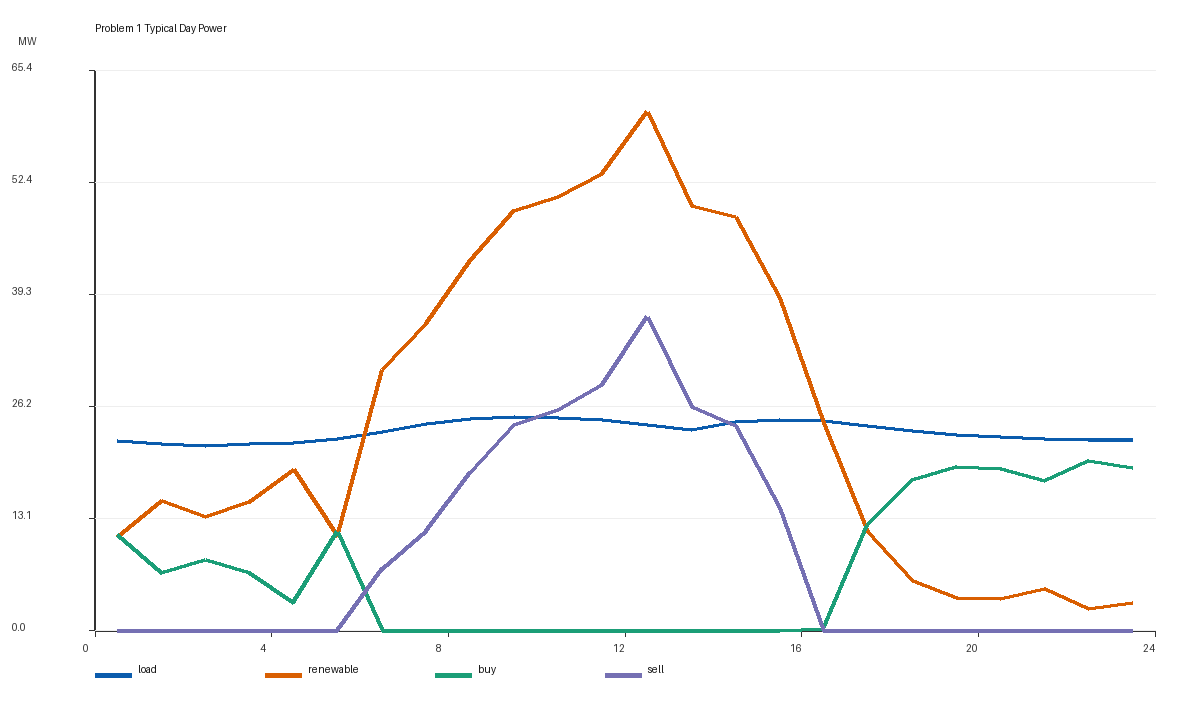
\includegraphics[width=.88\textwidth]{fig_problem1_power.png}
\caption{问题一典型日功率曲线}
\label{fig:p1-power}
\end{figure}

\subsection{问题二：离散开停机调度}
72 t/d 产能下，合成氨额定产量为 3 t/h。因此 72、63、54、45、36 t/d 分别对应 24、21、18、15、12 个开机小时。模型枚举可开机小时组合并选择综合成本最低方案。

\begin{table}[H]
\centering
\caption{问题二典型日不同产量结果}
\begin{tabular}{rrrrrrl}
\toprule
日产量 & 实际产量 & $r_1$ & $r_2$ & $r_3$ & 综合成本 & 分类 \\
\midrule
72 & 72.00 & 0.865 & 0.533 & 0.067 & 6265.44 & 全满足 \\
63 & 63.00 & 0.843 & 0.597 & 0.078 & 5380.97 & 全满足 \\
54 & 54.00 & 0.802 & 0.673 & 0.099 & 4653.00 & 全满足 \\
45 & 45.00 & 0.510 & 0.667 & 0.245 & 4018.62 & 部分满足 \\
36 & 36.00 & 0.105 & 0.597 & 0.447 & 3284.27 & 部分满足 \\
\bottomrule
\end{tabular}
\end{table}

典型日最低综合吨氨成本对应 36 t/d 方案，但其绿电指标仍为部分满足。这表明离散开停机可以降低运行成本，但不能自动解决新能源消纳结构问题。
\begin{figure}[H]
\centering
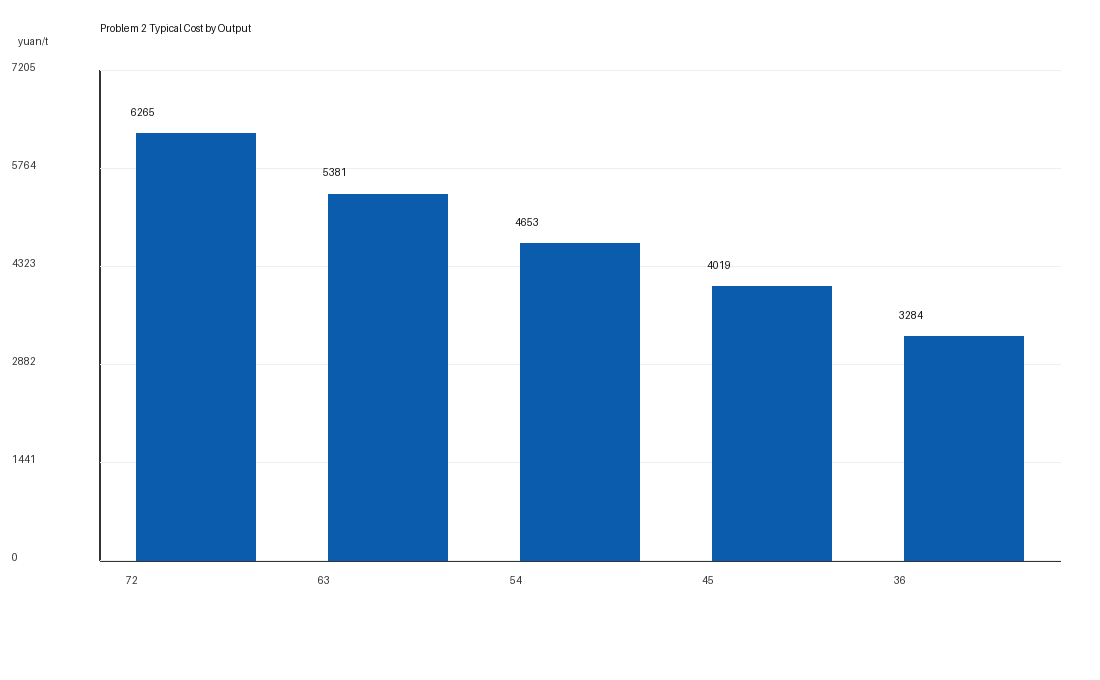
\includegraphics[width=.82\textwidth]{fig_problem2_typical_cost.png}
\caption{问题二典型日不同产量成本}
\end{figure}

\subsection{问题三：连续功率调节}
连续调节模型将日产量作为等式约束，并在 10\%--100\% 额定功率范围内分配小时制氨负荷。由于联网模式下电网可兜底，模型始终可行；优化方向是尽量将柔性负荷安排在低电价或高风光富余时段。

\begin{table}[H]
\centering
\caption{问题三 360 天代表年结果}
\begin{tabular}{rrrrrr}
\toprule
日产量 & 年产量 & 年均成本 & 全满足天数 & 部分满足天数 & 不满足天数 \\
\midrule
36 & 12960.00 & 4304.55 & 165 & 195 & 0 \\
45 & 16200.00 & 5084.19 & 240 & 120 & 0 \\
54 & 19440.00 & 5726.32 & 240 & 120 & 0 \\
63 & 22680.00 & 6466.04 & 300 & 60 & 0 \\
72 & 25920.00 & 7228.97 & 270 & 90 & 0 \\
\bottomrule
\end{tabular}
\end{table}

代表年最低年平均综合吨氨成本对应 36 t/d，成本为 4304.55 元/t。图 \ref{fig:p3-cost} 展示了不同日产量下的年均成本变化。
\begin{figure}[H]
\centering
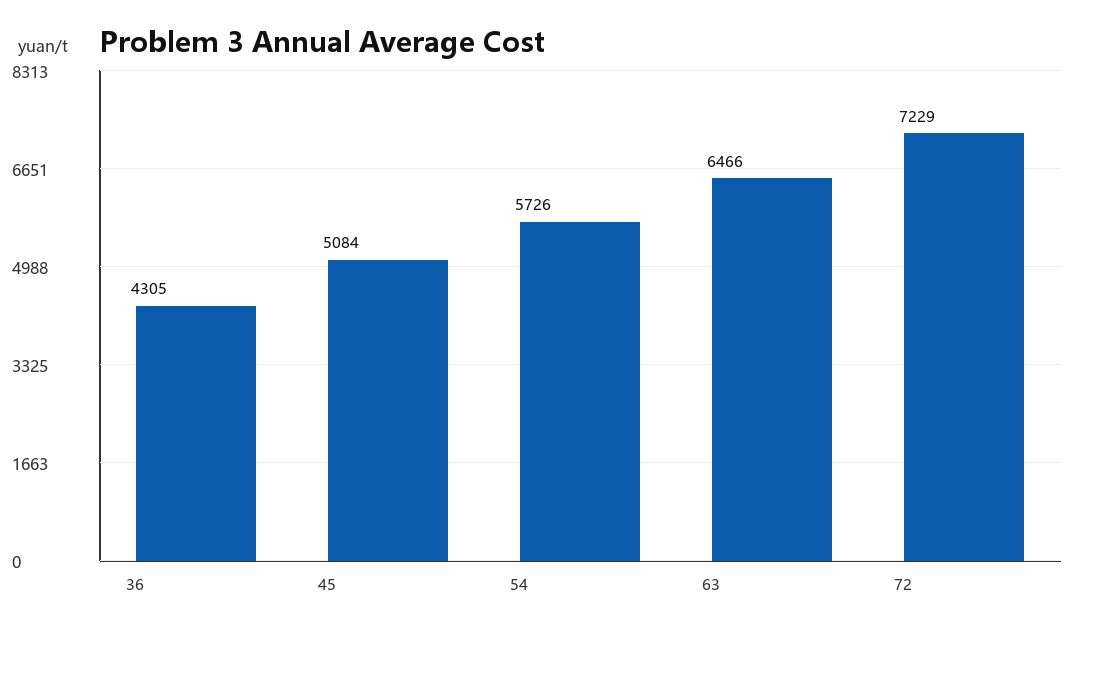
\includegraphics[width=.82\textwidth]{fig_problem3_annual_cost.png}
\caption{问题三不同产量代表年平均成本}
\label{fig:p3-cost}
\end{figure}

\subsection{问题四：离网储能配置}
离网模式下无购电和上网，储能调度需要满足功率平衡、SOC 上下界、SOC 首尾一致和充放电互斥。MILP 约束为
\begin{equation}
0.1q^{\max}u_t\le q_t\le q^{\max}u_t,
\end{equation}
\begin{equation}
SOC_{t+1}=(1-\lambda)SOC_t+\eta_{ch}P^{ch}_t-\frac{P^{dis}_t}{\eta_{dis}},\quad SOC_{24}=SOC_0.
\end{equation}
同时先最小化常规负荷缺供，再在该服务水平下最大化制氨量，防止模型通过牺牲常规负荷虚假提高产量。

最大弃电场景由无储能离网结果识别，为 风电场景4-光伏场景1。储能前后对比如表 \ref{tab:p4-compare}。
\begin{table}[H]
\centering
\caption{最大弃电场景储能前后对比}
\label{tab:p4-compare}
\begin{tabular}{lrr}
\toprule
项目 & 无储能 & 有储能 \\
\midrule
日产氨量/t & 46.19 & 47.74 \\
弃电量/MWh & 177.29 & 148.82 \\
常规负荷缺供/MWh & 0.000000 & 0.000001 \\
综合吨氨成本/(元/t) & 4256.93 & 4250.24 \\
\bottomrule
\end{tabular}
\end{table}

最终储能配置为 $E_{bat}=20.0$ MWh、$P_{bat}=5.0$ MW。回算 24 个场景后，代表年产氨量为 10064.49 t，年平均综合吨氨成本为 4240.87 元/t。求解器状态为 \texttt{pulp\_milp\_optimal}。
\begin{figure}[H]
\centering
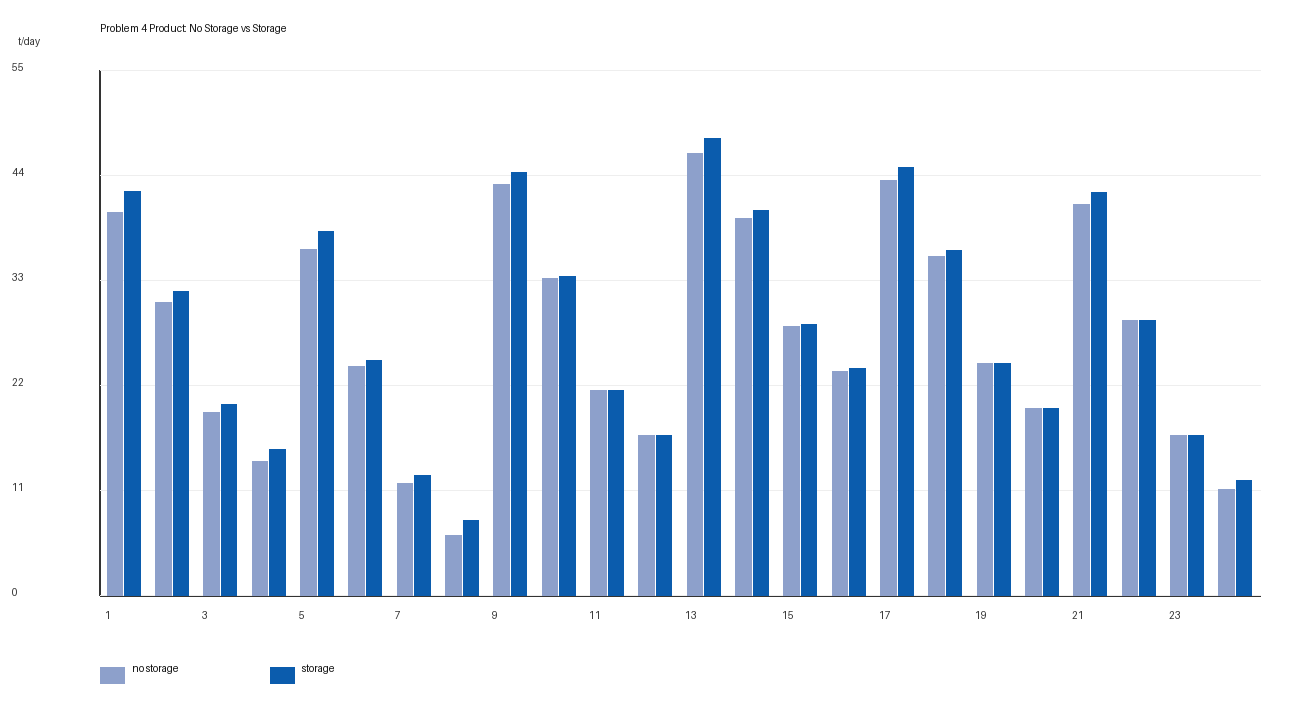
\includegraphics[width=.82\textwidth]{fig_problem4_storage_compare.png}
\caption{问题四储能前后各场景产量对比}
\end{figure}

\subsection{问题五：政策影响分析}
高渗透绿电直连园区的积极影响包括：促进新能源就近消纳，将波动性风光电转化为绿色氢氨等可储运产品，提高工业园区低碳竞争力。潜在风险包括：局部潮流波动增强、系统备用和调峰压力上升、多主体计量结算边界复杂化，以及低风光时段离网运行可靠性下降。

政策建议包括：坚持以荷定源，避免单纯追求新能源装机规模；将电解槽、合成氨装置和储能纳入统一灵活性资源管理；推动多用户园区化绿电直连交易，明确物理边界和责任边界；建立绿色氢氨认证与溯源体系；对提供调节能力的园区探索辅助服务补偿机制。

\section{模型的评价}
\subsection{模型的优点}
本文模型的优点在于：第一，问题一至四共用同一指标和成本函数，避免口径漂移；第二，严格区分题面阈值和政策背景阈值；第三，问题四通过 MILP 显式刻画设备启停、充放电互斥和 SOC 约束；第四，所有年化统计均按 360 天代表年计算，结果可复现。

\subsection{模型的不足}
模型仍存在若干不足：未考虑启停损耗、设备爬坡、最小连续开机时间和电解槽寿命折损；未引入储氢、卖氢和碳交易机制；风光场景只采用题面典型场景，未扩展到多年气象随机模拟。这些内容可作为后续灵敏度分析或工程深化方向。

\section{参考文献}
\begin{thebibliography}{9}
\setlength{\itemsep}{-2mm}
\bibitem{policy2025} 国家发展和改革委员会，国家能源局. 关于有序推动绿电直连发展有关事项的通知，2025.
\bibitem{policy2026} 国家发展和改革委员会，国家能源局. 有序推动多用户绿电直连发展有关事项的通知，2026.
\bibitem{model} 韩中庚. 数学建模方法及其应用[M]. 高等教育出版社, 2005.
\end{thebibliography}

\newpage
\appendix
\section{程序与复现说明}
本文完整可复现工程位于交付包 \texttt{reproduce/A\_solution}。其中 \texttt{src/run\_all.py} 为最终求解脚本，\texttt{data/raw} 包含题面 PDF 和 8 个原始附件。复现命令如下：
\begin{lstlisting}[language=bash]
cd reproduce
python -m pip install -r requirements.txt
python -X utf8 A_solution/src/run_all.py
\end{lstlisting}
主要输出包括 \texttt{outputs/tables} 中的 CSV 表、\texttt{outputs/A题\_求解结果汇总.xlsx}、\texttt{outputs/report/main.tex} 和 PDF 报告。

\section{验证结果}
\begin{longtable}{lll}
\toprule
检查项 & 数值 & 是否通过 \\
\midrule
xlsx\_count & 8 & True \\
hours & 24 & True \\
scenario\_count & 24 & True \\
problem2\_targets & 72,63,54,45,36 & True \\
problem3\_lp\_status & analytic\_optimal & True \\
scipy\_available & True & True \\
pulp\_available & True & True \\
strict\_milp\_solver\_available & True & True \\
problem4\_solver\_status & pulp\_milp & True \\
problem4\_storage\_e\_nonnegative & 20.0 & True \\
\bottomrule
\end{longtable}

\end{document}
